\chapter{Inleiding}

Op dit eigenste moment zijn er waarschijnlijk enkele honderden \emph{spiders} actief op internet.
Deze computerprogramma's, die soms ook \emph{robots} of \emph{wanderers} worden genoemd, reizen
het internet rond om bepaalde documenten -- in het bijzonder afbeeldingen -- te localiseren. Deze 
documenten worden ge\"indexeerd in een databank, die dan doorzocht kan worden door een zoekmachine. 

Zoekmachines zoals \emph{Google} en \emph{Yahoo} hebben op die manier reeds databanken
opgebouwd die meer dan een miljard afbeeldingen bevatten. Het wordt bijgevolg steeds belangrijker
om manieren te zoeken om deze gigantische collecties van afbeeldingen op een effeci\"ente wijze
te doorzoeken.


\section{Text-based image retrieval}

Alle belangrijke bestaande zoekmachines bieden \emph{text-based image retrieval} (TBIR) aan. 
Figuur~\ref{fig:tbir} toont de algemene architectuur van deze machines. Elke afbeelding 
wordt voorzien van tekstuele annotaties, zoals bijvoorbeeld de 
bestandsnaam of woorden uit de webpagina waarvan de afbeelding deel uitmaakt. Deze annotaties
worden gebruikt voor het indexeren van de afbeeldingen in de databank.

De gebruiker van een TBIR-systeem start een zoekactie door \'e\'en of meerdere trefwoorden door te geven
aan het systeem. Het systeem vergelijkt deze trefwoorden vervolgens met de annotaties uit
de databank. De afbeeldingen waarvan er annotaties overeenkomen met een trefwoord, maken
deel uit van het resultaat van de query. Men hoeft hiervoor uiteraard niet alle afbeeldingen
uit de databank te overlopen, vermits de databank ge\"indexeerd is op de annotaties. 

\section{Content-based image retrieval}

Omdat de tekst-gebaseerde aanpak in de praktijk dikwijls tekortschiet, is men op zoek gegaan 
naar manieren om het zoeken te baseren op de visuele inhoud van de afbeeldingen 
\cite{smeulders:cbir_end_of_early_years}. Zo zijn de \emph{content-based image retrieval} (CBIR) systemen 
\cite{veltcamp:cbirs} ontstaan. 
De algemene architectuur van een dergelijk systeem wordt ge\"illustreerd door
figuur~\ref{fig:cbir}. Men maakt gebruik van een proces dat 
\emph{(visual) feature extraction} genoemd wordt \cite{rui:image_retr}. Dit proces zet een afbeelding om in een 
\emph{feature vector}. Met behulp van multidimensionale indexering kan men deze kenmerkenvector
dan gebruiken als alternatief voor de tekstuele annotaties bij TBIR.

De meeste CBIR-systemen werken volgens het \emph{query-by-example} principe. Dit houdt in dat de
gebruiker een voorbeeld-afbeelding opgeeft, waarna het systeem op zoek gaat naar afbeeldingen
die visuele gelijkenissen vertonen met dit voorbeeld. Hiervoor wordt eerst de feature vector van
de opgegeven afbeelding bepaald, om deze vervolgens te vergelijken met de kenmerkenvectoren in
de databank. Het uiteindelijke resultaat bestaat uit de afbeeldingen uit de databank 
waarvan de overeenkomstige vectoren grote similariteit vertonen met de vector van de 
voorbeeld-afbeelding. Doordat de databank ge\"indexeerd is op de kenmerkenvectoren, kan men 
vermijden dat men hiervoor de volledige databank moet overlopen.

\begin{figure}[tb]
\begin{center}
\subfigure[]{
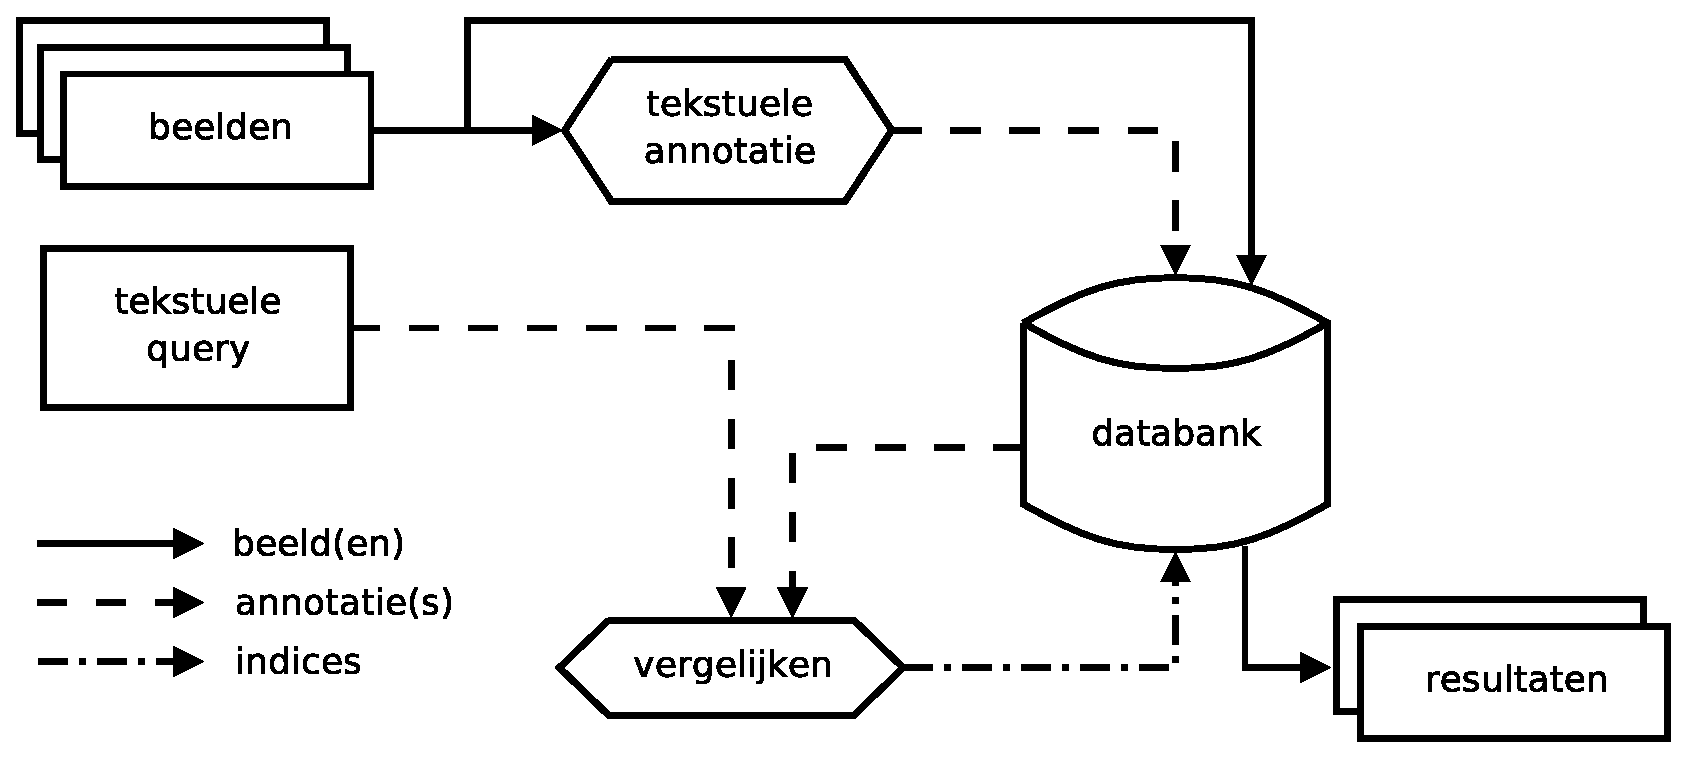
\includegraphics[width=10cm]{images/tbir.eps}
\label{fig:tbir}
}
\subfigure[]{
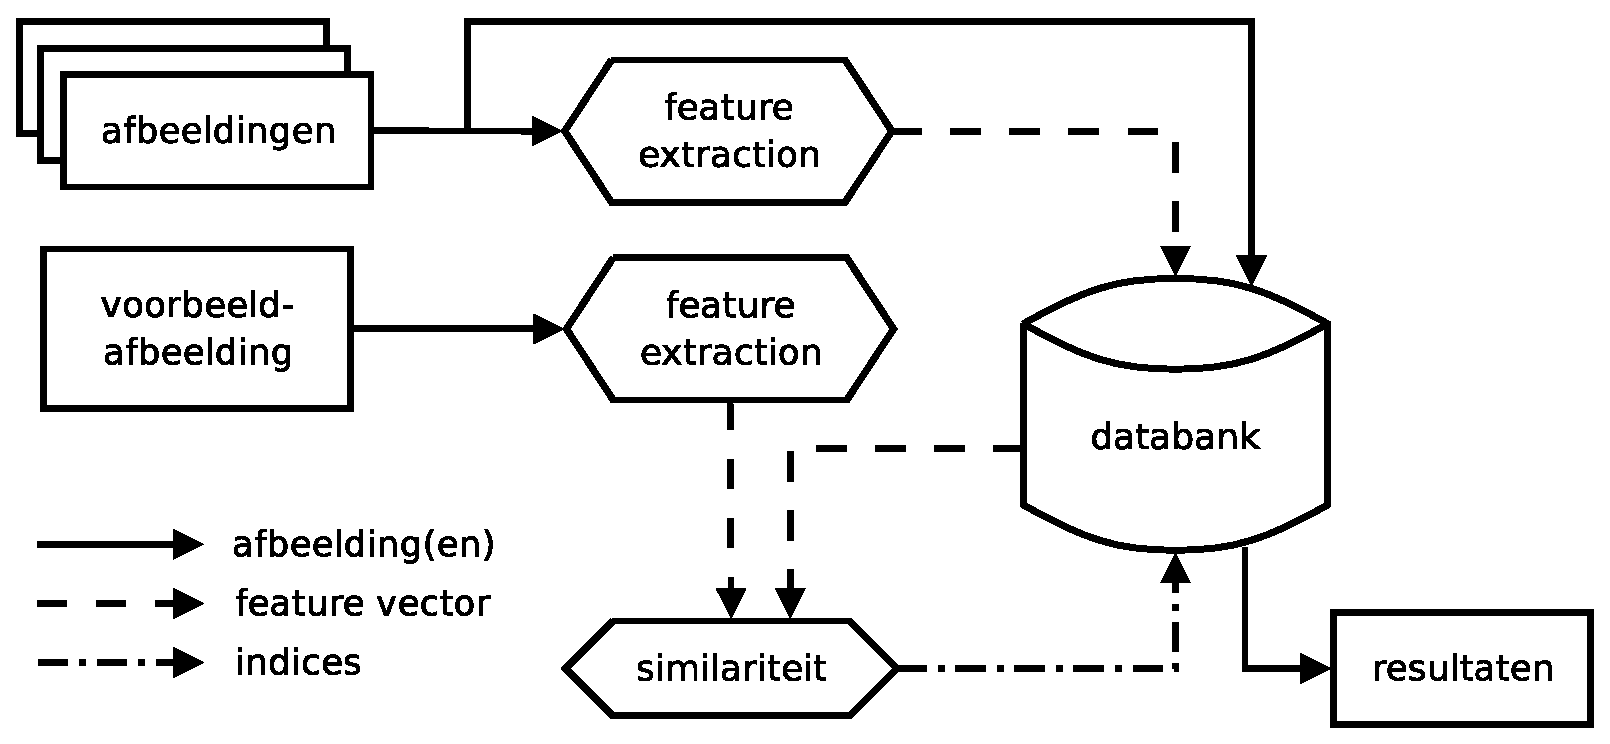
\includegraphics[width=10cm]{images/cbir.eps}
\label{fig:cbir}
}
\caption{\label{fig:cbir_en_tbir}Algemene architectuur van (a) een TBIR- en 
(b) een CBIR-systeem.}
\end{center}
\end{figure}

\section{Similariteitsgebaseerd rangschikken van de zoekresultaten}

Door hun grote complexiteit is het vrijwel onmogelijk om CBIR-systemen te gebruiken voor het 
doorzoeken van zeer omvangrijke databanken. Bovendien beschikt de gebruiker niet altijd over
een geschikte voorbeeld-afbeelding. Dit probleem kan eventueel nog opgelost worden door gebruik
te maken van een voorbeeld-schets, maar ook dat is in de praktijk niet altijd even handig.

Het is dus zinvol om te zoeken naar manieren om inhoud-gebaseerde aspecten toe te voegen aan
TBIR-systemen. De manier die we in deze scriptie bespreken is het 
similariteitsgebaseerd rangschikken van de resultaten van een TBIR-systeem. Hierbij verwachten we
nog steeds dat de gebruiker een tekstuele query opgeeft, waarop het systeem antwoordt met een 
lijst van afbeeldingen die overeenkomen met die query. Daarna heeft de gebruiker echter ook nog 
de mogelijkheid om een verzameling van voorbeeld-afbeeldingen te kiezen uit deze lijst. Het 
systeem zal er vervolgens voor zorgen dat de zoekresultaten gerangschikt worden in 
volgorde van similariteit met de voorbeeld-afbeeldingen.

